\chapter{Experimental Evaluation}
This chapter presents the procedure that is followed in order to provide the experimental evidences. Subsequently, the main findings are presented with appropriate explanation according to the Standard. 

\section{The experiment Set-Up}
The evaluation is carried out on Windows 8 with i7 CPU, 12GB Ram and a solid state disk (SSD). Also, the following versions of DBMSs had been installed: PostgreSQL Version 9.6, Microsoft SQL Server Express Edition 2016, IBM DB2 Express-C, Oracle Database 12c and MySQL Community Edition 5.7. 

A very large number of SQL queries are generated using the random query generator tool. More precisely, more than 100,000 queries are generated. In addition, different schemas are used varying from two to ten relations and two to ten attributes. Since the data types of attributes may be important, the following data types are used: TEXT, CHAR, VARCHAR, INTEGER, SMALLINT, BIGINT. Furthermore,  we generated data with different NULL rate such as 5\%, 10\%, 20\% and 40\% for identify if differences can arise depending on the number of NULLs that a database contains.  Furthermore, for each schema a database instance is generated using the random data generator Datafiller. As an important consideration that needs to be checked with these experiments is whether various features of the Standard are implemented identically, thus the instances size was 100 rows per table. It will be aimless to use larger size of instances since issues and differences of the Standard can be still disclose with a smaller size. In that way, the throughput of generated queries is increased and more queries can be evaluated in less time. 


\section{Experiment Results}
The implemented framework is used to conduct the experiments. In that way, the current implementation is checked and tested whether is capable to detect differences and issues between the five DBMSs. The results which are illustrated below have the following format: Firstly,  the SQL query that causes an error or a semantic issue is presented ( As may some features of the Standard are not implemented at all, or they are implemented differently). Then, a table for each query is provided which demonstrates if any DBMS raises an error,  otherwise, the keyword ‘Executed’ meaning that the SQL query is executed. Afterwards, a comprehensive explanation is given for each query by explaining about the source of the problem and an explanation according to the SQL standard is provided.   

 \begin{figure}        
      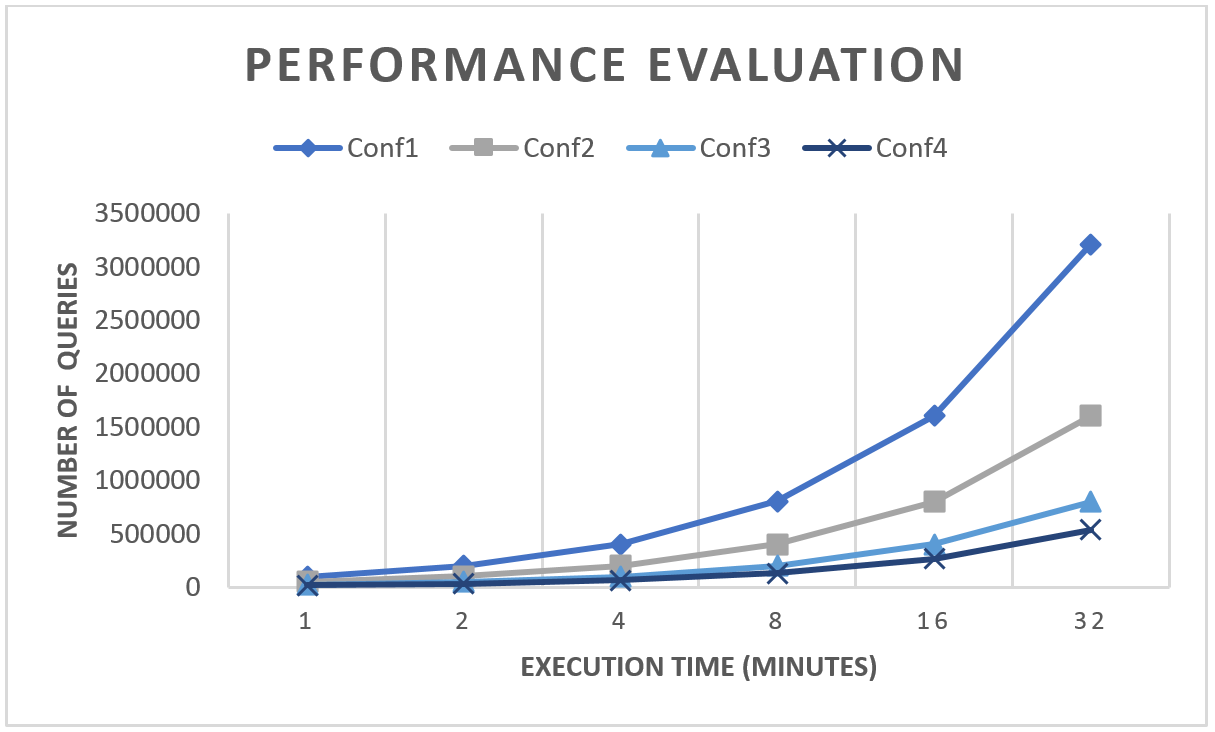
\includegraphics[width=\textwidth,height=8cm,width=10cm]{Images/performance_evaluation}
      \caption{Performance Evaluation}
      \label{fig:Performance Evaluation}
 \end{figure}

\hfill\newline\textbf{Difference 1:}
\hfill\newline\textbf{Q1:}
\begin{mdframed}[nobreak=true, backgroundcolor=lightgray!20] 
\begin{lstlisting}[style=SQL]
SELECT r41.A AS A0
FROM r4 AS r41
WHERE 1*1
\end{lstlisting}
\end{mdframed}

\begin{table}[h]
\centering
\caption{Difference 1}
\begin{tabular}{|p{2cm}|p{11.5cm}| }
\hline
\textbf{DBMS} & \textbf{Result Message}                                                                                                 \\ \hline
Mysql         & Works                                                                                                                   \\ \hline
PostgreSQL    & {[}42804{]} ERROR: argument of WHERE must be type boolean, not type integer                                             \\ \hline
MS Server     & {[}S0001{]}{[}4145{]} An expression of non-boolean type specified in a context where a condition is expected, near '1'. \\ \hline
Oracle        & {[}42000{]}{[}933{]} ORA-00933: SQL command not properly ended                                                          \\ \hline
IBM DB2       & Works                                                                                                                   \\ \hline
\end{tabular}
\end{table}

According to the Standard each expression in the ‘WHERE’ clause is evaluated to a boolean type such as True, False and Unknown. Thus, each row is evaluated to a boolean type and rows that returned true are included in the result. The Q1 performs multiplication between two constants in the ‘WHERE’ clause and cannot be evaluated to a boolean type, instead it should return an integer type. It is expected that the Q1 will raise an error if it is executed, nevertheless, Mysql and IBM DB2 execute the query without to raise any error. Although the expression in the ‘WHERE’ clause should return a boolean type, these two DBMSs convert an integer type to a boolean type. On the contrary with the rest three DBMSs which throw an exception.  

\hfill\newline\textbf{Difference 2:}
\hfill\newline\textbf{Q2:}
\begin{mdframed}[backgroundcolor=lightgray!20] 
\begin{lstlisting}[style=SQL]
SELECT r21.A AS A0 
FROM r2 AS r21
WHERE true
\end{lstlisting}
\end{mdframed}
 
 
\begin{table}[h]
\centering
\caption{Difference 2}
\label{my-label}
\begin{tabular}{|p{2cm}|p{11.5cm}| }
\hline
\textbf{DBMS} & \textbf{Result Message}                                                                                                   \\ \hline
Mysql         & Works                                                                                                                     \\ \hline
PostgreSQL    & Works                                                                                                                     \\ \hline
MS Server     & {[}S0001{]}{[}4145{]} An expression of non-boolean type specified in a context where a condition is expected, near 'true' \\ \hline
Oracle        & {[}42000{]}{[}920{]} ORA-00920: invalid relational operator                                                               \\ \hline
IBM DB2       & Works                                                                                                                     \\ \hline
\end{tabular}
\end{table}

As it is aforementioned, each expression in the ‘WHERE’ clause is evaluated to a boolean type. Thus, instead of having a specific expression, the keywords True/false can be specified which is the type that each expression is evaluated. As a consequence, it is reasonable to have the ‘True’ keyword in the WHERE clause indicating that each row selected in the ‘FROM’ clause will be included in the results. Nevertheless, Q2 raised an error if it is executed on Microsoft SQL  Server and Oracle DBMSs, in the contrast with the rest DBMS which the query is executed without to raise an error. With respect to SQL standard there is not explicit mention about the keyword true in the ‘WHERE’ Clause. 

\hfill\newpage

\hfill\newline\textbf{Difference 3:}
\hfill\newline\textbf{Q3:}
\begin{mdframed}[backgroundcolor=lightgray!20]
\begin{lstlisting}[style=SQL]
SELECT  NULL/NULL, 1/2, NULL-NULL
FROM r2 AS  r21, r4  AS  r41
WHERE  r41.B > r21.B 
\end{lstlisting}
\end{mdframed}

\begin{table}[h]
\centering
\caption{Difference 3}
\label{my-label}
\begin{tabular}{|p{2cm}|p{11.5cm}| }
\hline
\textbf{DBMS} & \textbf{Result Message}                                                                                                                                   \\ \hline
Mysql         & Works                                                                                                                                                     \\ \hline
PostgreSQL    & {[}42725{]} ERROR: operator is not unique: unknown / unknown Hint: Could not choose a best candidate operator. You might need to add explicit type casts. \\ \hline
Microsoft SQL Server     & Works                                                                                                                                                     \\ \hline
Oracle        & Works                                                                                                                                                     \\ \hline
IBM DB2       & Works                                                                                                                                                     \\ \hline
\end{tabular}
\end{table}

Boolean data type comprises the distinct truth values True and False. Apart from these values, boolean data type supports also the truth value Unknown as the NULL value. As a result, the Standard does not make a distinction between NULL value of the boolean data type and the truth value Unknown and based on the Standard a division between NULL should result to a NULL. The evaluation of the NULL/NULL in the Q3 should result to Unknown value. Nevertheless, PostgresSQL raises an error when executes this query, in the contrary with the rest DBMSs which are executed the query without any error. 


\hfill\newline\textbf{Difference 4:}
\hfill\newline\textbf{Q4:}

\begin{mdframed}[backgroundcolor=lightgray!20]
\begin{lstlisting}[style=SQL]
SELECT  r21.B/3
FROM  r2 AS r21, r4 AS r41
WHERE NOT(NOT(r41.A <> 18 ) )  
\end{lstlisting}
\end{mdframed}

 
\begin{table}[h]
\centering
\caption{Difference 4}
\label{my-label}
\begin{tabular}{|p{2cm}|p{11.5cm}| }
\hline
\textbf{DBMS} & \textbf{Result Message} \\ \hline
Mysql         & Works                   \\ \hline
PostgreSQL    & Works                   \\ \hline
MS Server     & Works                   \\ \hline
Oracle        & Works                   \\ \hline
IBM DB2       & Works                   \\ \hline
\end{tabular}
\end{table}

The Q4 is executed on Databases that contain smallint data type for the attribute r21.B. Thus, this query is executed without cause an error on any of five DBMSs. Nevertheless, the results differ slightly in terms of their return type. In DB2, PostgreSQL and MS Server the results for the column r21.B/3 are returned as integer type, on the contrary with MySQL and Oracle DBMSs where the results are returned as decimal data type. 

\hfill\newline\textbf{Difference 5:}
\hfill\newline\textbf{Q5:}

\begin{mdframed}[backgroundcolor=lightgray!20]
\begin{lstlisting}[style=SQL]
SELECT (MIN(r41.B) % AVG(r41.A) ) 
FROM r4 AS r41
WHERE (10 >= 19 )     
GROUP BY r41.A, r41.B
\end{lstlisting}
\end{mdframed}

\begin{table}[h]
\centering
\caption{Difference 5}
\label{my-label}
\begin{tabular}{|p{2cm}|p{11.5cm}| }
\hline
\textbf{DBMS} & \textbf{Result Message}                                \\ \hline
Mysql         & Works                                                  \\ \hline
PostgreSQL    & Works                                                  \\ \hline
MS Server     & Works                                                  \\ \hline
Oracle        & {[}22019{]}{[}911{]} ORA-00911: invalid ‘\%’ character \\ \hline
IBM DB2       & Works                                                  \\ \hline
\end{tabular}
\end{table}

An important consideration is that arithmetic operations such as addition, multiplications and  subtraction are supported in the SELECT clause. Another important arithmetic operation which is also supported in the ‘SELECT’ clause is the  (modulo). Nevertheless, the syntax of \% (modulo) operator differ in Oracle’s database. More precisely, Oracle database instead of using \% which is supported by the rest DBMSs, it uses a function called MOD. Thus, the Q5 needs to replace the operator \%  with function ‘mod’ in order to be syntactically correct in Oracle’s db, that is, MOD( MIN(r41.B), AVG(r41.A) ). 

\hfill\newpage

\hfill\newline\textbf{Difference 6:}
\hfill\newline\textbf{Q6:}
\begin{mdframed}[backgroundcolor=lightgray!20]
\begin{lstlisting}[style=SQL]
SELECT r41.A AS A0
FROM r4 AS r41
\end{lstlisting}
\end{mdframed}

\begin{table}[h]
\centering
\caption{Difference 6}
\label{my-label}
\begin{tabular}{|p{2cm}|p{11.5cm}| }
\hline
\textbf{DBMS} & \textbf{Result Message}                                        \\ \hline
Mysql         & Works                                                          \\ \hline
PostgreSQL    & Works                                                          \\ \hline
MS Server     & Works                                                          \\ \hline
Oracle        & {[}42000{]}{[}933{]} ORA-00933: SQL command not properly ended \\ \hline
IBM DB2       & Works                                                          \\ \hline
\end{tabular}
\end{table}

With respect to the Standard, alias feature is optional and it is not compulsory to be implemented in the modern DBMSs. The purpose of this feature is to rename tables or columns. Thus this feature can be used both with attributes in the ‘SELECT’ clause and for tables in the ‘FROM’ clause. Aliases are given using ‘AS’ keyword. In addition, it can be used to rename a subquery in the FROM clause and subsequently to access it using its alias. The Oracle’s database support to use ‘AS’ when defining column aliases, but it does not allow use ‘AS’ when defining table aliases (in the ‘FROM’ clause), on the contrary with the rest DBMSs which support the alias feature both to rename tables or columns. 


\hfill\newline\textbf{Difference 7:}
\hfill\newline\textbf{Q7:}

\begin{mdframed}[backgroundcolor=lightgray!20]
\begin{lstlisting}[style=SQL]
(SELECT r41.A AS A0
 FROM r4 AS r41 ) 
EXCEPT ALL
(SELECT r21.A AS A0
 FROM r2 AS r21, r4 AS r42 )
\end{lstlisting}
\end{mdframed}

\begin{table}[h]
\centering
\caption{difference 7}
\label{my-label}
\begin{tabular}{|p{2cm}|p{11.5cm}| }
\hline
\textbf{DBMS} & \textbf{Result Message}                                                                                                                                                 \\ \hline
Mysql         & {[}42000{]}{[}1064{]} You have an error in your SQL syntax; check the manual that,corresponds to your MySQL server version for the right syntax to use near 'EXCEPT ALL \\ \hline
PostgreSQL    & Works                                                                                                                                                                   \\ \hline
MS Server     & S0002{]}{[}324{]} The 'ALL' version of the EXCEPT operator is not supported.                                                                                            \\ \hline
Oracle        & {[}42000{]}{[}933{]} ORA-00933: SQL command not properly ended                                                                                                          \\ \hline
IBM DB2       & Works                                                                                                                                                                   \\ \hline
\end{tabular}
\end{table}

\hfill\\\\
EXCEPT ALL is an optional feature according to the Standard. The usage of this feature is to return all rows from the outer query which are not present in the inner query without removing the duplicates. Thus, this operator is fully supported by the Standard but it is optional meaning that it is not compulsory to be implemented by modern DBMSs. MySql and Oracle database do not support this operator. Nevertheless, Oracle, supports the same operator but with different name called ‘MINUS ALL’ keyword. As a result, MINUS ALL  has exactly the same behaviour on Oracle’s database with the EXCEPT ALL.  Lastly, PostgreSQL and IBM DB2 support the EXCEPT ALL operator. 


\hfill\newline\textbf{Difference 8:}
\hfill\newline\textbf{Q8:}

\begin{mdframed}[backgroundcolor=lightgray!20]
\begin{lstlisting}[style=SQL]
(SELECT r41.A AS A0
 FROM r4 AS r41, r2 AS r21, r3 AS r31
 WHERE NOT(r31.B <> r41.A ) )
EXCEPT
(SELECT r21.A AS A0
 FROM r2 AS r21, r4 AS r41
 WHERE r41.A <> r41.B )
\end{lstlisting}
\end{mdframed}

\begin{table}[h]
\centering
\caption{Difference 8}
\label{my-label}
\begin{tabular}{|p{2cm}|p{11.5cm}|}
\hline
\textbf{DBMS} & \textbf{Result Message}                                                                                                                                             \\ \hline
Mysql         & {[}42000{]}{[}1064{]} You have an error in your SQL syntax; check the manual that corresponds to your MySQL server version for the right syntax to use near 'EXCEPT \\ \hline
PostgreSQL    & Works                                                                                                                                                               \\ \hline
MS Server     & Works                                                                                                                                                               \\ \hline
Oracle        & {[}42000{]}{[}933{]} ORA-00933: SQL command not properly ended                                                                                                      \\ \hline
IBM DB2       & Works                                                                                                                                                               \\ \hline
\end{tabular}
\end{table}

\hfill\\\\\\
‘EXCEPT’ is a mandatory feature according to the Standard and all DBMSs must support this feature in order to comply to the Standard. The usage of this feature results to return all rows from the outer query which are not present in the inner query with removing the duplicates. Only MySQL does not support the ‘EXCEPT’ even though it is a compulsory feature according to the Standard.. Nevertheless, Oracle database instead of use  ‘EXCEPT’ as keyword, it uses ‘MINUS’ which has an identical behavior. The rest DBMSs support this operator. 


\hfill\newline\textbf{Difference 9:}
\hfill\newline\textbf{Q9:}

\begin{mdframed}[backgroundcolor=lightgray!20]
\begin{lstlisting}[style=SQL]
(SELECT r41.A AS A0
 FROM r4 AS  r41, r3 AS r31
 WHERE (NULL <= 6 OR NOT(r31.B <> r41.A ) ) )
INTERSECT ALL
(SELECT r21.A AS A0
 FROM r2 AS r21, r4 AS r41
 WHERE r41.A <> r41.B OR ( 0 <> 14)  AND r41.A > r21.B)
\end{lstlisting}
\end{mdframed}

 
\begin{table}[h]
\centering
\caption{Difference 9}
\label{my-label}
\begin{tabular}{|p{2cm}|p{11.5cm}| }
\hline
\textbf{DBMS} & \textbf{Result Message}                                                                                                                                          \\ \hline
Mysql         & {[}42000{]}{[}1064{]} You have an error in your SQL syntax; check the manual that corresponds to your MySQL server version for the right syntax to use near 'ALL \\ \hline
PostgreSQL    & Works                                                                                                                                                            \\ \hline
MS Server     & {[}S0001{]}{[}324{]} The 'ALL' version of the INTERSECT operator is not supported.                                                                               \\ \hline
Oracle        & {[}42000{]}{[}928{]} ORA-00928                                                                                                                                   \\ \hline
IBM DB2       & Works                                                                                                                                                            \\ \hline
\end{tabular}
\end{table}

\hfill\newpage
With respect to the Standard INTERSECT ALL is an optional feature. The usage of this feature is to return all the rows which are presented in both inner and outer queries result, and without removing duplicates. MySQL, Microsoft SQL Server and oracle do not support this feature at all. On the contrary, PostgreSQL and IBM DB2 support this feature. 

 
\hfill\newline\textbf{Difference 10:}
\hfill\newline\textbf{Q10:}

\begin{mdframed}[backgroundcolor=lightgray!20]
\begin{lstlisting}[style=SQL]
SELECT  7/0 AS ART0, 1%NULL AS ART1
FROM r1 AS r11
WHERE (NULL = 19 AND r11.b <> 5)   
\end{lstlisting}
\end{mdframed}
  
\begin{table}[h]
\centering
\caption{Difference 10}
\label{my-label}
\begin{tabular}
{|p{2cm}|p{11.5cm}| }
\hline
\textbf{DBMS} & \textbf{Result Message}                                 \\ \hline
Mysql         & Works                                                   \\ \hline
PostgreSQL    & {[}22012{]} ERROR: division by zero                     \\ \hline
MS Server     & {[}S0001{]}{[}8134{]} Divide by zero error encountered. \\ \hline
Oracle        & ORA-01476: divisor is equal to zero                     \\ \hline
IBM DB2       & {[}22012{]}{[}-801{]} Division by zero was attempted..  \\ \hline
\end{tabular}
\end{table}

A division with zero should not allowed  according to the Standard and it should  always raise an error. Nevertheless, MySQL does not raise an error and the result of the division with zero is NULL. 


 
\hfill\newline\textbf{Difference 11:}
\hfill\newline\textbf{Q11:}

\begin{mdframed}[backgroundcolor=lightgray!20]
\begin{lstlisting}[style=SQL]
SELECT r11.a AS A1, r11.b AS A2
FROM r1 AS r11
WHERE (r11.b, r11.a) IN (SELECT r12.a AS A4, r12.b AS A3
                         		 FROM r1 AS r12)
\end{lstlisting}
\end{mdframed}

\begin{table}[h]
\centering
\caption{Difference 11}
\label{my-label}
\begin{tabular}{|p{2cm}|p{11.5cm}|}
\hline
\textbf{DBMS} & \textbf{Result Message}                                                                                                 \\ \hline
Mysql         & Works                                                                                                                   \\ \hline
PostgreSQL    & Works                                                                                                                   \\ \hline
MS Server     & {[}S0001{]}{[}4145{]} An expression of non-boolean type specified in a context where a condition is expected, near ','. \\ \hline
Oracle        & Works                                                                                                                   \\ \hline
IBM DB2       & Works                                                                                                                   \\ \hline
\end{tabular}
\end{table}

A division with zero should not allowed  according to the Standard and it should  always raise an error. Nevertheless, MySQL does not raise an error and the result of the division with zero is NULL. 


\hfill\newline\textbf{Difference 12:}
\hfill\newline\textbf{Q12:}

\begin{mdframed}[backgroundcolor=lightgray!20]
\begin{lstlisting}[style=SQL]
SELECT  r31.b AS A1
FROM r3 AS r31
WHERE r31.a >= r31.a
GROUP BY r31.a
\end{lstlisting}
\end{mdframed}
 
\begin{table}[h]
\centering
\caption{Difference 12}
\label{my-label}
\begin{tabular}{|p{2cm}|p{11.5cm}| }
\hline
\textbf{DBMS} & \textbf{Result Message}                                                                                                                                                                                                                                                                 \\ \hline
Mysql         & Works                                                                                                                                                                                                                                                                                   \\ \hline
PostgreSQL    & {[}42803{]} ERROR: column "r31.b" must appear in the GROUP BY clause or be used in an aggregate function Position: 9                                                                                                                                                                    \\ \hline
MS Server     & {[}S0001{]}{[}8120{]} Column 'r3.B' is invalid in the select list because it is not contained in either an aggregate function or the GROUP BY clause.                                                                                                                                   \\ \hline
Oracle        & {[}42000{]}{[}979{]} ORA-00979: not a GROUP BY expression                                                                                                                                                                                                                               \\ \hline
IBM DB2       & {[}42803{]}{[}-119{]} An expression starting with "B" specified in a SELECT clause, HAVING clause, or ORDER BY clause is not specified in the GROUP BY clause or it is in a SELECT clause, HAVING clause, or ORDER BY clause with a column function and no GROUP BY clause is specified \\ \hline
\end{tabular}
\end{table}

According to the Standard, only columns that appear in the ‘GROUP BY’ clause can be selected. The intuition behind this issue is based on the fact that if non-grouped and non-aggregate fields are selected, then the DBMSs cannot know which field to return. The Q12 project the attribute  ‘r31.b’ which is not appear in the the ‘GROUP BY’ clause. PostgreSQL, Microsoft SQL Server, Oracle and IBM DB2 raise an error as the attribute does not appear in the ‘GROUP BY’ clause. Nevertheless, MySQL executes the query without to raise an error. 



\hfill\newline
\hfill\newline\textbf{Difference 13:}
\hfill\newline\textbf{Q13:}

\begin{mdframed}[backgroundcolor=lightgray!20]
\begin{lstlisting}[style=SQL]
SELECT  NULL+NULL AS ART1
FROM r4 AS r41, r5 AS r51
WHERE  r41.a >= r41.a OR ( r41.a >= 4 )
GROUP BY r41.a
HAVING MIN(r41.a) < 7506
\end{lstlisting}
\end{mdframed}

\begin{table}[h]
\centering
\caption{Difference 13}
\label{my-label}
\begin{tabular}{|p{2cm}|p{11.5cm}| }
\hline
\textbf{DBMS} & \textbf{Result Message}                                                                                                                                  \\ \hline
Mysql         & Works                                                                                                                                                    \\ \hline
PostgreSQL    & {[}42725{]} ERROR: operator is not unique: unknown + unknown Hint: Could not choose a best candidate operator. You might need to add explicit type casts \\ \hline
MS Server     & Works                                                                                                                                                    \\ \hline
Oracle        & Works                                                                                                                                                    \\ \hline
IBM DB2       & Works                                                                                                                                                    \\ \hline
\end{tabular}
\end{table}

The Standard does not make a distinction between NULL value of the boolean data type and the truth value Unknown and based on the Standard an addition between two NULLs should result to a NULL. The evaluation of the NULL+NULL in the Q13 should result to Unknown value. Nevertheless, PostgresSQL raises an error when executes this query, in the contrary with the rest DBMSs which are executed the query without any error. 


\hfill\newpage
\hfill\newline\textbf{Difference 14:}
\hfill\newline\textbf{Q14:}

\begin{mdframed}[backgroundcolor=lightgray!20]
\begin{lstlisting}[style=SQL]
SELECT  'SQL' || 'STANDARD'
FROM R1
\end{lstlisting}
\end{mdframed}
 
\begin{table}[h]
\centering
\caption{Difference 14}
\label{my-label}
\begin{tabular}{|p{2cm}|p{11.5cm}| }
\hline
\textbf{DBMS} & \textbf{Result Message}                         \\ \hline
Mysql         & Works                                           \\ \hline
PostgreSQL    & Works                                           \\ \hline
MS Server     & {[}S0001{]}{[}102{]} Incorrect syntax near '|'. \\ \hline
Oracle        & Works                                           \\ \hline
IBM DB2       & Works                                           \\ \hline
\end{tabular}
\end{table}

According to the Standard, concatenation is a mandatory feature and it should be supported by all DBMSs with a double-pipe mark ‘||’. The purpose is to concatenate two or more strings into one. Thus, executing Q14 is expected the result to be ‘SQLSTANDARD’. Nevertheless, MySQL supports the double pipe operator, but it treats the double-pipe “||” as a logical OR and thus the query returns 0. MySQL uses the CONCAT() function as concatenation and it takes as parameters one or more strings.   Microsoft SQL Server uses the ‘+’ operator in order to perform the concatenation. Oracle and PostgreSQL support the double-pipe ‘||’ concatenation operator. 




\hfill\newline\textbf{Difference 15:}
\hfill\newline\textbf{Q15:}

\begin{mdframed}[backgroundcolor=lightgray!20]
\begin{lstlisting}[style=SQL]
SELECT  *
FROM  r1 AS R1 , r1 AS R1
\end{lstlisting}
\end{mdframed}

\begin{table}[h]
\centering
\caption{Difference 15}
\label{my-label}
\begin{tabular}{|p{2cm}|p{11.5cm}| }
\hline
\textbf{DBMS} & \textbf{Result Message}                                                                       \\ \hline
Mysql         & {[}42000{]}{[}1066{]} Not unique table/alias: 'R1'                                            \\ \hline
PostgreSQL    & {[}42712{]} ERROR: table name "r1" specified more than once                                   \\ \hline
MS Server     & {[}S0001{]}{[}1011{]} The correlation name 'R1' is specified multiple times in a FROM clause. \\ \hline
Oracle        & {[}42000{]}{[}933{]} ORA-00933: SQL command not properly ended                                \\ \hline
IBM DB2       & Works                                                                                         \\ \hline
\end{tabular}
\end{table}

Q15 should raise an error because it give the same alias on two tables. Thus, it will be unambiguous to which table it is referred. Nevertheless, the query is executed on IBM DB2 database, where on the rest DBMSs raise an error. 


\hfill\newline\textbf{Difference 16:}
\hfill\newline\textbf{Q16:}

\begin{mdframed}[backgroundcolor=lightgray!20]
\begin{lstlisting}[style=SQL]
SELECT TRIM('    SQLSTANDARD    ')
FROM R1;
\end{lstlisting}
\end{mdframed}

\begin{table}[h]
\centering
\caption{Difference 16}
\label{my-label}
\begin{tabular}{|p{2cm}|p{11.5cm}| }
\hline
\textbf{DBMS} & \textbf{Result Message}                                                  \\ \hline
Mysql         & Works                                                                    \\ \hline
PostgreSQL    & Works                                                                    \\ \hline
MS Server     & {[}S00010{]}{[}195{]} 'TRIM' is not a recognized built-in function name. \\ \hline
Oracle        & Works                                                                    \\ \hline
IBM DB2       & Works                                                                    \\ \hline
\end{tabular}
\end{table}

\hfill\newpage
According to Standard trim function is a mandatory feature and it should be implemented by all DBMSs. The usage of trim feature is that it returns the string which is given as argument with leading and/or trailing pad character. This function is supported by most of DBMSs, except Microsoft SQL Server. 


\hfill\newline\textbf{Difference 17:}
\hfill\newline\textbf{Q17:}

\begin{mdframed}[backgroundcolor=lightgray!20]
\begin{lstlisting}[style=SQL]
SELECT  2 * 5 AS ART
WHERE ( 1 = 1 )
WHERE r1.c3 LIKE 'standard%'
\end{lstlisting}
\end{mdframed}


\begin{table}[h]
\centering
\caption{Difference 17}
\label{my-label}
\begin{tabular}{|p{2cm}|p{11.5cm}| }
\hline
\textbf{DBMS} & \textbf{Result Message}                                                                                                                                                     \\ \hline
Mysql         & {[}42000{]}{[}1064{]} You have an error in your SQL syntax; check the manual that corresponds to your MySQL server version for the right syntax to use near 'WHERE (1 = 1 ) \\ \hline
PostgreSQL    & Works                                                                                                                                                                       \\ \hline
MS Server     & Works                                                                                                                                                                       \\ \hline
Oracle        & {[}42000{]}{[}923{]} ORA-00923: FROM keyword not found where expected                                                                                                       \\ \hline
IBM DB2       & {[}42601{]}{[}-104{]} Expected tokens may include: "FROM"                                                                                                                   \\ \hline
\end{tabular}
\end{table}

The basic structure of an SQL query is ‘SELECT...FROM...WHERE’. The Q17 omits the ‘FROM’ clause. SQL query without ‘FROM’ clause can be executed only on PostgreSQL and Microsoft SQL Server. On the contrary, Mysql, Oracle and IBM DB2 raises an error. 


\hfill\newpage

\hfill\newline\textbf{Difference 18:}
\hfill\newline\textbf{Q18:}

\begin{mdframed}[backgroundcolor=lightgray!20]
\begin{lstlisting}[style=SQL]
SELECT  SUBSTRING ('Standard', 1, 4)
FROM  R1
\end{lstlisting}
\end{mdframed}

\begin{table}[h]
\centering
\caption{Difference 18}
\label{my-label}
\begin{tabular}{|p{2cm}|p{11.5cm}| }
\hline
\textbf{DBMS} & \textbf{Result Message}                                         \\ \hline
Mysql         & Works                                                           \\ \hline
PostgreSQL    & Works                                                           \\ \hline
MS Server     & Works                                                           \\ \hline
Oracle        & {[}42000{]}{[}904{]} ORA-00904: "SUBSTRING": invalid identifier \\ \hline
IBM DB2       & Works                                                           \\ \hline
\end{tabular}
\end{table}

The substring function is a mandatory feature according to the Standard and as a result all DBMSs should implement this feature. The usage of substring is to return a part of the string which given as argument. Mysql, PostgreSQL, IBM DB2 and Microsoft Sql Server support this function. Oracle database use Substr instead of Substring which has a similar behaviour. The prototype of oracle’s function is as follow: $substr (column_name, start_pos , no_of_characters).$ 


\hfill\newline\textbf{Difference 19:}
\hfill\newline\textbf{Q19:}

\begin{mdframed}[backgroundcolor=lightgray!20]
\begin{lstlisting}[style=SQL]
SELECT "SQLSTANDARD"
FROM R1
\end{lstlisting}
\end{mdframed}

 
\begin{table}[h]
\centering
\caption{Difference 19}
\label{my-label}
\begin{tabular}{|p{2cm}|p{11.5cm}| }
\hline
\textbf{DBMS} & \textbf{Result Message}                                                        \\ \hline
Mysql         & Works                                                                          \\ \hline
PostgreSQL    & {[}42703{]} ERROR: column "SQLSTANDARD" does not exist Position: 8             \\ \hline
MS Server     & {[}S0001{]}{[}207{]} Invalid column name 'SQLSTANDARD'.                        \\ \hline
Oracle        & {[}42000{]}{[}904{]} ORA-00904: "SQLSTANDARD": invalid identifier              \\ \hline
IBM DB2       & {[}56098{]}{[}-727{]} An error occurred during implicit system action type "2" \\ \hline
\end{tabular}
\end{table}

\hfill\newpage
According to the SQL standard encompass by ‘. It is demonstrated in Q19 that MySQL allow a string to be encompassed by both ‘ and “ which make the SQL code less portable as the rest DBMSs raise an error if it is used “ instead if ‘. 


\hfill\newline\textbf{Difference 20:}
\hfill\newline\textbf{Q20:}

\begin{mdframed}[backgroundcolor=lightgray!20]
\begin{lstlisting}[style=SQL]
SELECT *
FROM r1 AS R1
WHERE R1.c3 = ’’’
\end{lstlisting}
\end{mdframed}
 
\begin{table}[h]
\centering
\caption{Difference 20}
\label{my-label}
\begin{tabular}{|p{2cm}|p{11.5cm}| }
\hline
\textbf{DBMS} & \textbf{Result Message} \\ \hline
Mysql         & Works                   \\ \hline
PostgreSQL    & Works                   \\ \hline
MS Server     & Works                   \\ \hline
Oracle        & Works                   \\ \hline
IBM DB2       & Works                   \\ \hline
\end{tabular}
\end{table}


The Q20 is executed on all DBMSs without to raise an error, though the semantic of this query differs. As it was mentioned in the background chapter, and more precisely in the missing value, Oracle database treats the empty string as NULL, on the contrary with the rest DBMSs, which treats it as a normal String. Thus, all the comparisons in the ‘WHERE’ clause involving NULL are evaluated to Unknown which implies that the result will be empty as none of the rows will be satisfied.  On the other hand, if there is at least a row which contains an empty string by executing the above query will be returned in the result. All the DBMSs except Oracle Database return in the result all the rows that contains an empty string in the column c3 and Oracle Database return an empty result. 



\hfill\newline\textbf{Difference 21:}
\hfill\newline\textbf{Q21:}

\begin{mdframed}[backgroundcolor=lightgray!20]
\begin{lstlisting}[style=SQL]
SELECT *
FROM R1
WHERE r1.c3 LIKE 'standard%'
\end{lstlisting}
\end{mdframed}


\begin{table}[h]
\centering
\caption{Difference 21}
\label{my-label}
\begin{tabular}{|p{2cm}|p{11.5cm}| }
\hline
\textbf{DBMS} & \textbf{Result Message} \\ \hline
Mysql         & Works                   \\ \hline
PostgreSQL    & Works                   \\ \hline
MS Server     & Works                   \\ \hline
Oracle        & Works                   \\ \hline
IBM DB2       & Works                   \\ \hline
\end{tabular}
\end{table}

Q21 is executed on all DBMSs without to raise an error but it differs semantically.  This query will not return the same results on all DBMSs. More precisely, all the tested systems contain a database that stores a field with the word ‘STANDARD’ (in capital letters) in the attribute c3 of the relation r1. By executing this query, it can be observed that some of the DBMSs are case sensitive with the LIKE operator. PostgreSQL and Oracle are case-sensitive, resulting to return an empty set. On the contrary with the rest systems, which returns one row which is the row that contains the word ‘STANDARD’ in the attribute c3.  




